\documentclass{article}
\usepackage[T1]{fontenc}
\usepackage{multirow}
\usepackage{mathtools}
\usepackage{changepage}
\usepackage{graphicx}
\usepackage[top=2.5cm,bottom=2.5cm,left=2cm,right=2cm]{geometry}
\newcommand{\arr}[1]{\rightarrow{q}}

\title{Report - Assignment 4}
\date{December 10, 2017}
\author{Romain Jufer}
\begin{document}

\maketitle

\section{Implementation}
To implement the algorithm we first note that a convolution can be splitted in two parts. We can first compute for each pixels the sum of itself with its two neighbors. Then we apply the same process for the columns. This idea is to avoid doing unecessary work by grouping the operations. To see this, consider a square of side 3 pixels. We count 1 operations everytime we store or add a value into the output. For the naive approach, where for each pixels we fetch all the neighbors and add them, we get a total of 9*9=81 operations to get the output. If we split the algorithm as we just said, we have 3 operations per pixels when we apply the "row" parts of the algorithm. Hence we have 3 * 3 pixels/row * 3 rows = 27 operations. We also have 27 operations for the "column" parts. This will give us a total of 27 + 27 = 54 operations. Therefore we get the same result but using 6/10 of the number of operations used in the naive version. \\

Using the concept we just described, we naturally divid the algorithm into two kernels representing the "row" and "column" computation. We now talk about the way we divide the data into blocks and threads per blocks. According to the specification of the K40 Accelerator used on SCITAS, we cannot have more than 1024 threads per block and a warp has a size of 32 threads. Therefore the best candidate we found by experimentation is having 32 threads in x-dimension and 32 in y-dimension resulting in 1024 threads in a block. The number of blocks is defined in both x-,y-directions as the length of our data devided by the number of threads. According to the specification we can have $2^{31}$ as the number of blocks in the x-direction and $2^{16}$ in the y-direction. This will clearly be enough for our case. \\

We tried to use shared memory for the implementation. First we loaded all the data needed, namely the pixels in the block plus the apron region of pixels around the block in a shared memory. Then we compute the output using the data in the shared memory. In theory it should have improved the runtime because the shared memory is faster than the global memory by approximately a factor of 100. However in practice it was not the case. One explanation might be that the number of access done in the shared memory is not large enough to compensate the overhead induced by filling the shared memory. If we were using more than just the direct neighbors of a pixels (e.g 3 pixels in each direction) this might become a faster solution. \\

Finally there might be runtime differences running first the kernel on the rows and then the columns or vice versa due to banking. Therefore we will provide the results for both in the next section.

\section{Runtime Results}
We note that we the runtimes for the GPU include the memory transfers. \\ \\
\begin{tabular}{|c|c|c|c|c|}
\hline
 & 100 by 100 array & 100 by 100 array & 1000 by 1000 array & 1000 by 1000 array \\
 & 10 iteration & 1000 iterations & 100 iterations & 10000 iterations \\
 \hline
 CPU baseline & 0.00015s & 0.02121s & 0.1488s & 21.87s \\
 \hline
 CPU optimized 16 cores & 0.000545s & 0.01761s & 0.02309 & 2.61s \\
 \hline
 GPU "rows then columns" & 0.1663s & 0.1783s & 0.2035s & 2.955s  \\
 \hline
 GPU "columns then rows" & 0.1625s & 0.1818s & 0.2043s & 2.973s \\
\hline
\end{tabular}
\newpage
We also show runtimes for larger size and more iterations to have an idea when the GPU baseline would take over the optimized multithreaded version. \\ \\
\begin{tabular}{|c|c|c|}
\hline
& 4096 by 4096 array & 8192 by 8192 array \\
& 5000 iterations & 1000 iterations \\
\hline
CPU optimized 16 cores & 36.83s & 20.97s \\
\hline
GPU "rows then columns" & 23.03s & 19.77s \\
\hline
\end{tabular}
\section{GPU Runtime Breakdown}
The breakdown is only given in percentage of the total runtime. The integers in the x-axis correspond to the specified configurations written below.
\begin{center}
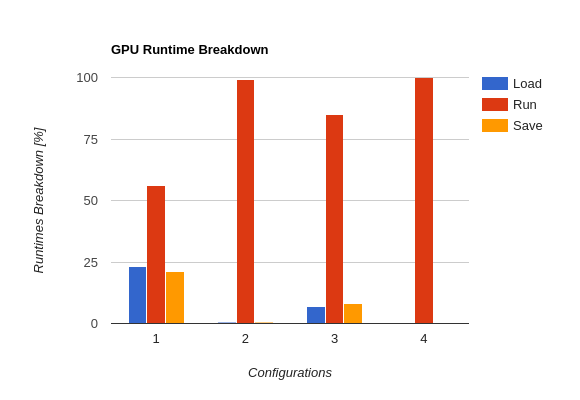
\includegraphics[scale=0.6]{graph.png}
\end{center}
Configurations
\begin{enumerate}
\item 100x100 array with 10 iterations
\item 100x100 array with 1000 iterations
\item 1000x1000 array with 100 iterations
\item 1000x1000 array with 10000 iterations
\end{enumerate}
\section{Analysis}
By the graph above, we can clearly see that, as the number of iterations grows, the overhead due to moving the data to/from the GPU becomes less significant. Refering to the runtime table we see that the GPU algorithm run faster than the baseline by a factor of ~7.35 in the fourth configuration. However, we need larger array with more iterations to really see a difference between the CPU multithreaded version and the GPU baseline. In the second table of runtimes we see that the GPU outrun the CPU version by a factor of 1.6 in the first configuration and by a factor of 1.06 in the second. Hence we see that both the size of the data and the number of operations need to be taken into account when designing a solution. Futhermore we cannot claim that the GPU algorithm cannot be further optimized using more complex techniques. In conclusion, the GPU is really powerful on large computation but easily beaten on "small" ones. Therefore we have to find through exprimentation and analysis, the threshold above which a GPU algorithm becomes superior.
\end{document}